\section{Les réseaux de neurones artificiels}
\label{chap4.section7}
Revenons au modèle de régression logistique de la section \ref{chap4.section6}, maintenant au lieu de le voir comme un modèle à part entière je vous suggère de penser à ce modèle comme une simple unité de calcul, une petite partie d'un modèle beaucoup plus grand. C'est assez peu commun d'expliquer les résaux neuronaux de cette manière mais c'est bien là les fondements de cet algorithme.

\begin{figure}
    \centering
    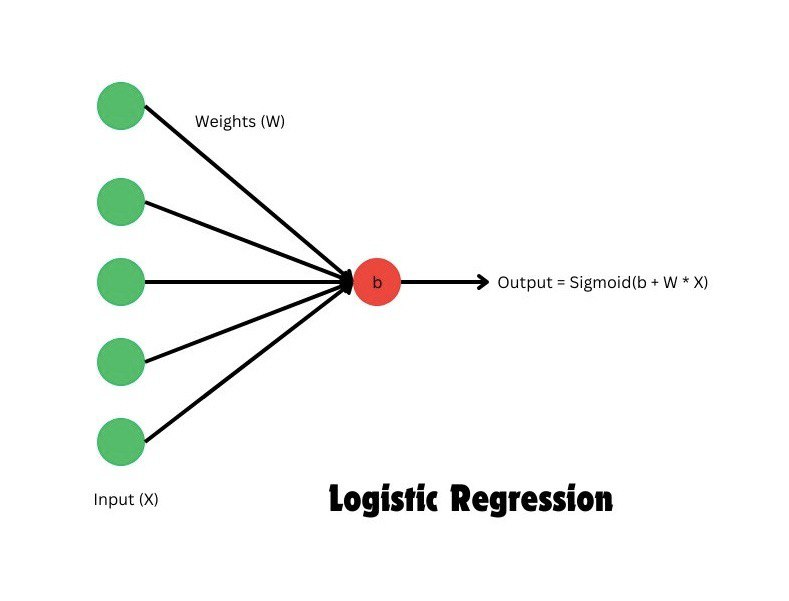
\includegraphics[width=0.75\linewidth]{images/logitReg2.png}
    \caption{Un modèle de régression logistique vu comme un neuronne}
    \label{fig:fig9}
\end{figure}

Les réseaux de neuronnes artificiels sont un type de modèle paramétriques qui marche grâce à la superposition de plusieurs couches de petites unités de calcul qui sont traversées une à une par les différents attributs \(x_{j,i}\) d'un exemple de donnée \(x_j\). Les sorties d'une couche devenant les entrées de la suivante jusqu'à une couche de sortie représentant la prédiction du modèle pour l'exemple \(x_j\) (cette couche peut aussi contenir plusieurs unités de calculs). Ce sont les fondements de toute une famille d'algorithmes basés sur ce concept et d'un sous domaine de l'apprentissage automatique appélé: \textbf{Apprentissage profond}\footnote{L'apprentissage profond est un sous domaine de l'apprentissage qui utilise des réseaux neuronaux artificiels et d'autres algorithmes compexes pour simuler le pouvoir de décision complexe du cerveau humain. Ce genre de modèle alimente la majeure partie de l’intelligence artificielle aujourd’hui.}.

Les unités de calcul vont être appélées « neuronnes » et le type de modèle que je décris dans le paragraphe précédent est le type de modèle d'apprentissage profond le plus simple appélé: réseau neuronal à action directe ou \textbf{feedforward neural network}. Comme je l'ai dit dans la section \ref{chap4.sec6.sub2}, l'implémentation que j'ai fait de la régression logistique était faite ainsi dans le but de faciliter l'analogie et la transition aux réseaux de neuronnes. En effet si l'on considère un modèle de régression logistique comme un seul neuronne unique comme l'illustre la figure \ref{fig:fig9}, il dévient beaucoup plus simple de raisonner avec les réseaux neuronaux à action directe,  vous pouvez les voir comme des modèles qui superpose plusieurs modèles de régression logistique (neuronnes) par couche. La figure \ref{fig:fig10} montre un réseau neuronal directe avec 2 couches intermédiaires ou couches cachées \textit{(hidden layers)} et un seul neuronne de sortie pensé pour la classification binaire.

\begin{figure}
    \centering
    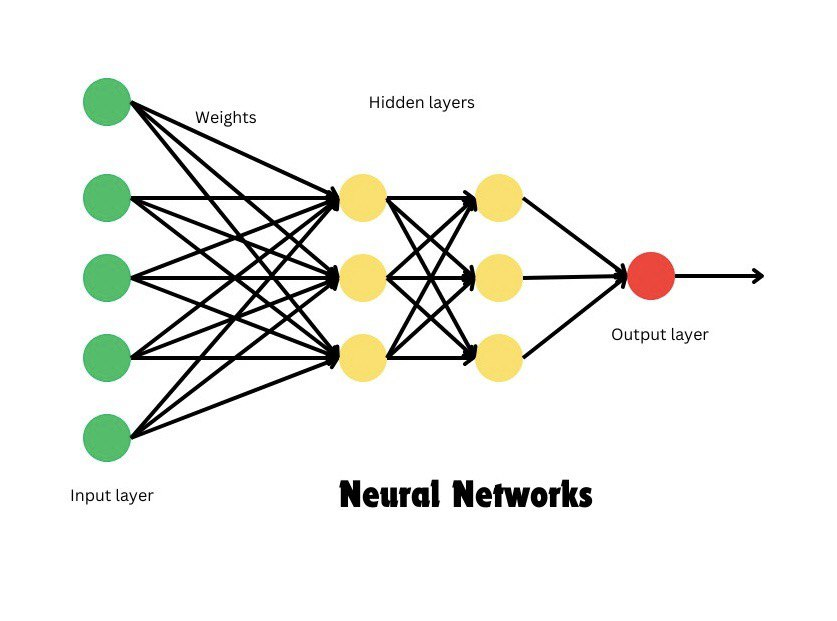
\includegraphics[width=0.75\linewidth]{images/neuralnet.png}
    \caption{Un réseau neuronal à action directe vu comme un ensemble de modèle de régression logistique}
    \label{fig:fig10}
\end{figure}

Ajoutez à celà le fait qu'on a la possibilité de remplacer la fonction sigmoid par toute autre fonction pour chaque neuronne en théorie (même si en pratique et par covention les neuronnes de la même couche utilisent la même fonction) et on a toutes les bases de l'apprentissage profond. Pour un neuronne la fonction qui permet de passer de \(\hat{y}_j = b + \Sigma_i w_i \cdot x_{j,i}\) à l'entrée du prochain neuronne est ce qu'on appelle une \textbf{fonction d'activation}. Pour simplifier les démonstrations dans ce document on va supposer que toutes les fonctions d'activations sont la fonction sigmoid.

\subsection{La rétro-propagation}
\label{chap4.sec7.sub1}
La rétro-propagation est une variante de l'algorithme de descente de gradient qui vise à adapter cette dernière à l'entraînement de réseaux de neuronnes multi-couches (\cite{nielse2018nneural}). L'algorithme est presque identique à la descente de gradient, juste qu'il apporte un support pour calculer les gradients des poids et des bias qui n'appartienne pas au neuronne de la couche de sortie en propageant l'erreur de la dernière couche aux précédentes grâce à ses gradients, d'où le non \textbf{rétro-propagation}. L'algorithme de rétro-propagation appliqué au poids et au bias du neuronne de sortie qui prédit la probabilité qu'un exemple \(x_j\) appartienne à la classe positive revient à la descente de gradient sur un modèle de régression logistique.

Avez vous pris soins de remarquer cette expression dans la section \ref{chap4.sec6.sub2}? \[\frac{\partial}{\partial w_i} L2 = \frac{\partial L2}{\partial Sigmoid(\hat{y}_j)} \cdot \frac{\partial Sigmoid(\hat{y}_j)}{\partial \hat{y}_j} \cdot \frac{\partial \hat{y}_j}{\partial w_i}\] Cette décomposition est connu sous le nom de: \textbf{règle de la chaîne des gradients} et elle est le fondement de l'algorithme de rétro-propagation car en interpolant ainsi des termes qui font le lien entre la fonction de perte et un poids ou un bias donné on peut trouver les expressions des gradients de fonction de perte par rapport à n'importe quel poids ou bias du réseau neuronal. L'algortihme de rétro-propagation appliqué aux couches cachées du réseau revient donc simplement à suivre la chaîne. Ce qui est en revanche très fastidieux puisque la chaîne s'aggrandit au fur et à mésure qu'on remonte dans le réseau. 

Tout cela paraît assez complexe pour quelqu'un qui n'est pas particulièrement bon en math et croyez moi j'ai souffert pour en arriver à ce petit niveau de compréhension. En résumé, la seule réelle différence entre l'algorithme de rétro-propagation et la descente de gradient est la taille de la chaîne des gradients. Les autres étapes une fois qu'on a les gradients de la fonction de perte par rapport à tous les poids et tous les bias restent identiques à la descente de gradient vu dans la section \ref{chap4.sec5.sub2}.

\subsection{Implémentation}
\label{chap4.sec7.sub2}
Comme dit précédemment, j'ai fait une implémentation avec keras d'un réseau de neuronnes à action directe. Après plusieurs tests, l'architecture qui conciliait les performances et le temps d'entraînement du modèle est composée d'une seule couche cachée de 100 neuronnes et d'une couche de sortie avec un seul neuronne. Les neuronnes de la couche cachée ont comme fonction d'activation la fonction d'unité linéaire rectifiée (\textbf{relu}) définie comme: \[relu(z) = max(0, z)\] En plus d'introduire une forme de non linéarité dans le fonctionnement du modèle, la fonction d'unité linéaire rectifiée et ses variantes sont généralement préférées pour les couches cachées en raison de la simplicité de leurs gradients ce qui permet d'accélerer considérablement la descente de gradient.

Pour l'unique neuronne de sortie, cela va de soit, la fonction sigmoid s'impose pour que les prédictions finales du modèle puisse être interprêtées comme la probabilité d'un exemple donnée de faire défaut sur son prêt. Et puisque le problème reste une classification binaire la fonction de coût reste la même que pour la régression logistique à savoir \textbf{log-loss}. Le meilleur modèle a été entraîner pour 10 époques d'entraînement sur des lots de 64 exemples par descente de gradient et avec un taux d'apprentissage de 0,001 encore une fois (\cite{diarra2024notebooks}).